\section{Results}
\subsection{Primary frozen synthetic holdout}
Table~\ref{tab:primary} and Fig.~\ref{fig:primary} show the paired comparison on exactly the same 15 queues. The candidate recovered 18 additional expert top-20 incidents and recalled 10 additional incidents in the first 20 groups. P@10 rose by six credited positions. These are absolute differences of 6.00, 3.33, and 4.00 percentage points, respectively; no statistical significance claim is made.
\begin{table*}[t]\centering\footnotesize\caption{Frozen paired holdout results. Fractions use evaluator opportunity denominators. Differences are candidate minus baseline; percentage differences are percentage points.}\label{tab:primary}\begin{tabularx}{\textwidth}{@{}Yrrr@{}}\toprule Metric & Frozen baseline & Endpoint fallback & Difference\\\midrule Incident Recall@20 & 250/300 (83.33\%) & 260/300 (86.67\%) & +10 (+3.33 pp)\\ Group recoverability & 263/300 (87.67\%) & 281/300 (93.67\%) & +18 (+6.00 pp)\\ P@10 & 107/150 (71.33\%) & 113/150 (75.33\%) & +6 (+4.00 pp)\\ Grouped-pair precision & 19,459/19,459 (100\%) & 20,117/20,117 (100\%) & 0 pp\\ False grouped pairs & 0 & 0 & 0\\ Mixed groups & 0 & 0 & 0\\\bottomrule\end{tabularx}\end{table*}

\begin{figure*}[t]\centering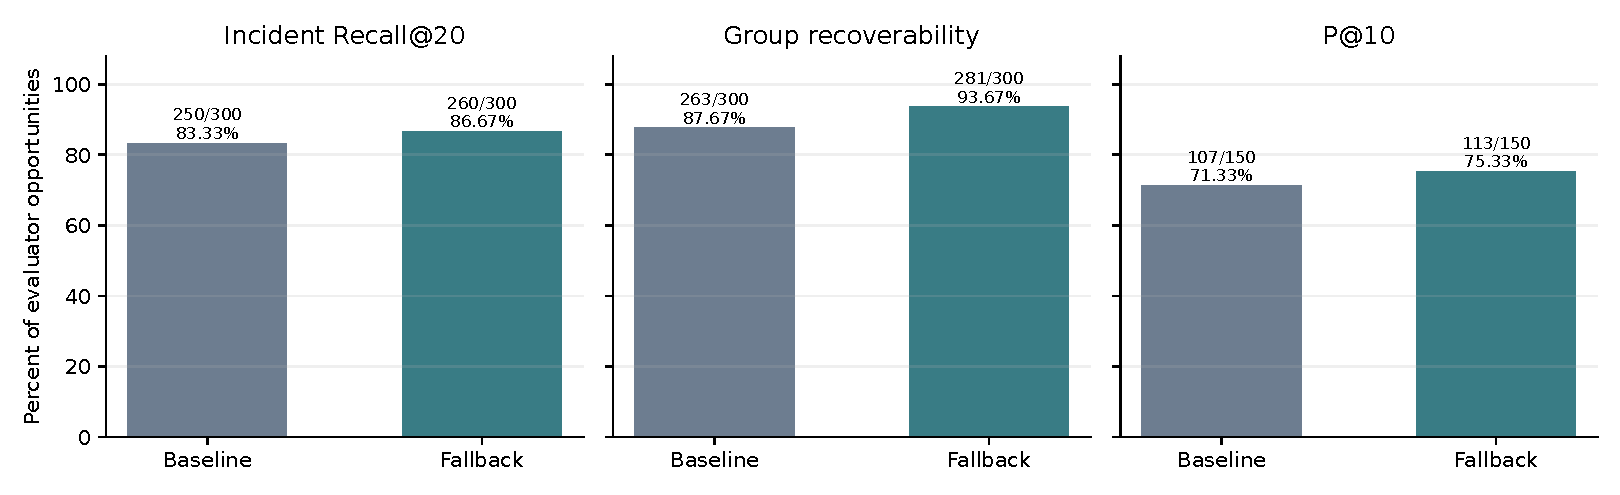
\includegraphics[width=.83\textwidth]{figures/phase33_results.pdf}\caption{Frozen synthetic holdout metrics from the verified summary, with exact counts and denominators. Zero-based axes permit direct comparison; the three panels have different evaluation opportunities and must not be summed.}\label{fig:primary}\end{figure*}
The simulator-truth audit classified all 28 newly accepted fallback unions and all 711 total candidate accepted unions as genuine. It recorded 150 false relationship-token rejections and 35 genuine-token abstentions. These token counts refer to a different evaluation unit than pair precision. Fig.~\ref{fig:safety} displays the all-group safety results; all 15 queues had zero false pairs and zero mixed groups in both arms. Queue-level Recall@20 nevertheless fell by one incident in two queues, and P@10 fell in two queues. Aggregate gains therefore do not imply uniform queue gains.

\begin{figure}[ht]\centering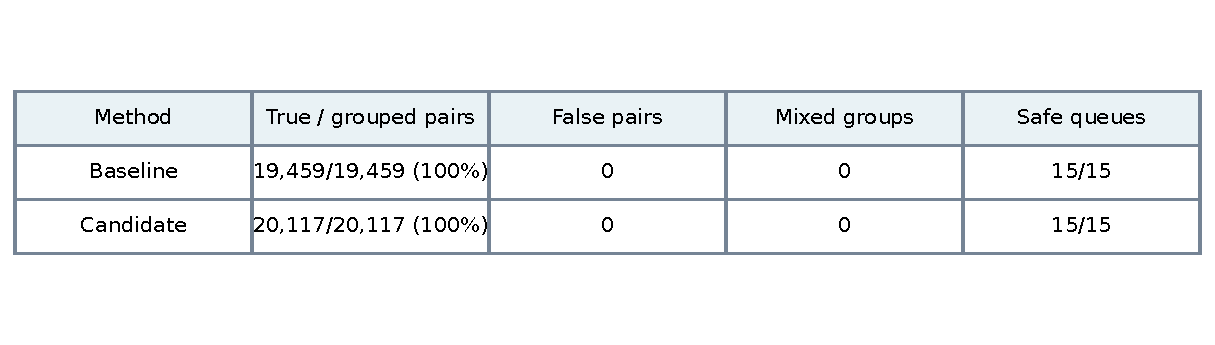
\includegraphics[width=.9\linewidth]{figures/safety_results.pdf}\caption{Grouped-pair and mixed-group outcomes on the 15-queue controlled holdout. Pair precision uses all within-group pairs; the count of safe queues is based on zero false grouped pairs and zero mixed groups in each queue. Zero observed errors under simulator truth is not a bound on real-world error rates.}\label{fig:safety}\end{figure}
\subsection{Decision confusion matrix and paired outcomes}
The post-evaluation truth audit of the candidate verifier records the exact relationship-token decision matrix in Table~\ref{tab:confusion}. An accepted token is a positive decision; a rejected token is a negative decision. The 711 accepted tokens include 28 additional fallback unions, all genuine under simulator truth. The 35 rejected genuine tokens quantify abstention caused by the strict evidence requirements; the 150 rejected false tokens show that false proposals were blocked. These decisions are \emph{token-level} observations, not all possible alert pairs and not the incident-retrieval confusion matrix. The audited token set contains 896 decisions. Its conditional token acceptance precision is $711/(711+0)=100\%$, genuine-token acceptance recall is $711/(711+35)=95.31\%$, and false-token rejection specificity is $150/(150+0)=100\%$. These are descriptive simulator-truth figures, not operational performance estimates.
\begin{table}[t]
\centering\caption{Candidate token-decision confusion matrix on the frozen synthetic holdout; truth opened only after predictions were sealed. Rows are verifier decisions; columns are simulator truth.}\label{tab:confusion}
\begin{tabular}{@{}lrr@{}}\toprule
 & Genuine relation & False relation\\\midrule
Accepted & \gaincell{711 (TP)} & 0 (FP)\\
Rejected/abstained & 35 (FN) & \gaincell{150 (TN)}\\\bottomrule
\end{tabular}
\end{table}
The incident-level matched-outcome table uses a different unit: the 300 expert top-20 incident opportunities. Fifteen were retrieved only by the candidate, five only by the baseline, and 245 by both, giving the net gain of ten (Table~\ref{tab:paired}). Because this population contains only designated positives, a conventional incident-level true-negative count or classification accuracy cannot be inferred. Likewise, grouped-pair recall requires a denominator for all same-incident eligible pairs; it is not supplied by the holdout summary. We do not manufacture these metrics from grouped-pair precision.
\begin{table}[t]
\centering\caption{Paired incident retrieval at rank 20 (300 expert opportunities).}\label{tab:paired}
\begin{tabular}{@{}lrr@{}}\toprule
 & Candidate recalled & Candidate missed\\\midrule
Baseline recalled & 245 & 5\\
Baseline missed & \gaincell{15} & 35\\\bottomrule
\end{tabular}
\end{table}
The frozen summary additionally reports nDCG@20 of 0.8852 versus 0.9201 and MRR of 1.0 in both arms. It records 1,333 versus 1,305 predicted groups and 683 versus 711 accepted merges. Its recorded run durations of 0.696 and 0.656 seconds are single execution measurements, with no repeated-run uncertainty or hardware-normalized latency claim.
\subsection{Where the aggregate gains arose}
The queue-level heatmap in Figure~\ref{fig:queueheat} displays integer candidate-minus-baseline differences rather than a smoothed trend. Recall increased in eight queues, was unchanged in five, and decreased by one in two. Recoverability increased in twelve queues and was unchanged in three; it did not decrease in this holdout. P@10 increased in five queues, was unchanged in eight, and decreased in two. Thus a positive aggregate result coexists with local retrieval losses. The per-queue denominator is 20 for Recall@20 and recoverability, and 10 for P@10.
\begin{figure*}[t]\centering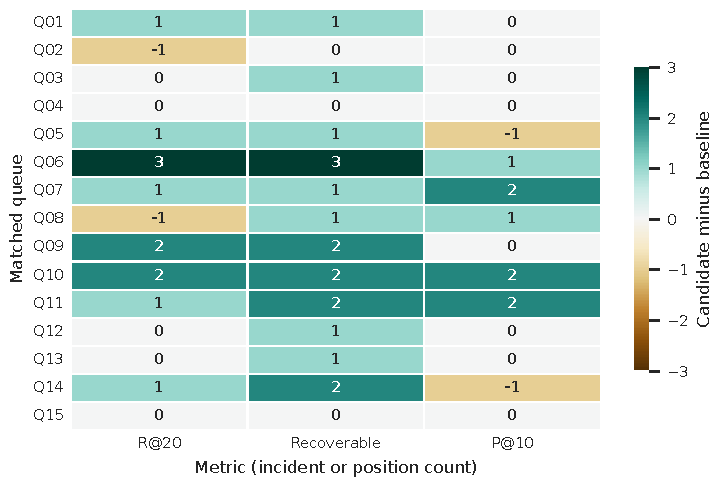
\includegraphics[width=.76\textwidth]{figures/queue_delta_heatmap.pdf}\caption{Per-queue change on the paired synthetic holdout. Each cell is candidate minus baseline, from the archived queue CSV. Blue-green marks gains, brown losses and white no change; printed integers remain readable without color. Queue numbering is display order, not a time series.}\label{fig:queueheat}\end{figure*}
Figure~\ref{fig:decomp} separates the reconstruction and ranking conditions for the 300 expert top-20 incident opportunities. The baseline's 263 recoverable incidents comprise 250 retrieved within the first 20 groups and 13 with a qualifying group outside that range. The candidate's 281 recoverable incidents comprise 260 retrieved and 21 outside. Consequently, the fallback reduced the number without any qualifying group from 37 to 19, while the number recoverable but not retrieved rose from 13 to 21. This arithmetic does not identify a causal ranking failure for an individual incident: the group partition and resulting score order both change under the fallback. It does show why recoverability cannot be substituted for Recall@20.
\begin{figure}[ht]\centering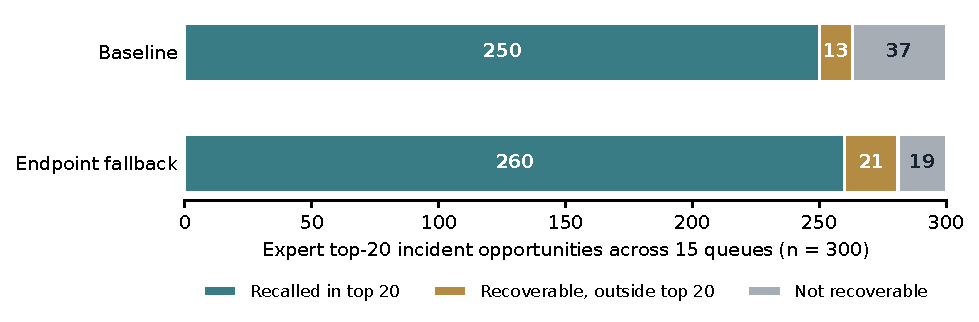
\includegraphics[width=.94\linewidth]{figures/retrieval_decomposition.pdf}\caption{Mutually exclusive status of the 300 expert top-20 incident opportunities under each frozen method: qualifying group ranked within 20, qualifying group only outside 20, or no qualifying group. Counts are derived from the archived aggregate recall and recoverability numerators. The bars are descriptive totals under the evaluator's 80\% completeness and purity qualification; they are not independent incident-level paired transitions.}\label{fig:decomp}\end{figure}

\subsection{Development-only and historical evidence}
Table~\ref{tab:development} summarizes separate ranking and evidence studies. Later development scores are not substituted for the frozen holdout or construed as a performance trajectory. The earlier historical synthetic holdout had 407/600 Recall@20 and 451/600 recoverability on another population; its scores are not directly comparable. An unsafe richer-claim development configuration produced 2,580 false pairs and 22 mixed groups, whereas independent-claim verification on that development cohort preserved zero false pairs and recovered 166/200 incidents.
\begin{table*}[t]\centering\footnotesize\caption{Later investigations on distinct development-only cohorts. B and C are matched within each row; they are not comparable across rows as successive improvements.}\label{tab:development}\begin{tabularx}{\textwidth}{@{}p{0.19\textwidth}Yrrr@{}}\toprule Study & Question & Baseline R@20 & Candidate R@20 & Candidate recoverability\\\midrule Ranking feature study & Post-group score & 264/300 & 267/300 & 277/300\\ Near-boundary rank study & Reorder below first ten & 258/300 & 258/300 & 273/300\\ Evidence-aware rank study & Visible evidence features & 265/300 & 262/300 & 277/300\\ Evidence availability & Frozen condition, stress tests & 257/300 & --- & 267/300\\ Hard-negative rank study & Pairwise trained reordering & 263/300 & 262/300 & 279/300\\\bottomrule\end{tabularx}\end{table*}
